%Projects
%--------
%
%An essential part of this course are the take-home projects.
%
%Instructions for the take-home exams:
%
% Reports can be done individually or in groups of two. However, reasonably open
% discussions of the assignments with other students in this course are
% acceptable, but must be acknowledged in the report. The reports should consist
% of two to five pages plus supplementary graphs, tables, program listings, etc.,
% and should be organized as follows:
%
% Introduction and Problem Background. Briefly describe the general problem you
% want to solve and why a numerical or computational solution (as opposed to an
% exclusively analytical solution) is required.
%
% Numerical Considerations. Briefly discuss the specific methods, software or
% algorithms you selected for this problem. Mention any specific features of
% MATLAB you exploited.
%
% Results.  Include a concise tabular or graphical presentation of the results.
% Every table and figure should have a caption and a title, and the axes of every
% plot should be clearly marked, so that the reader can understand the figures or
% plots without referring to the main text. All codes should be clearly
% documented, especially input and output parameters, if any, and a description
% of what the code does.
%
% Analysis. Include a solid discussion and analysis of the results presented.
% The discussion should address any difficulties you encountered, appropriate
% measures of performance (such as errors and computer time) and the apparent
% sources of error you observed.
%
% Lessons Learned. Elaborate a critical evaluation of the software you used. Make
% a list of the specific things you  learned by working out the assignment, both
% theoretical and practical issues.
%
% Acknowledgements. Mention discussions with other students or teachers, software
% downloaded from the web or  copied from a book, and any other relevant
% information you find fit to disclose.
%
% The grade you obtain will reflect whether or not you have correctly and
% efficiently solved the problem, and whether or not you adequately address the
% relevant theoretical and practical issues. A grade of 8-12 indicates work that
% is acceptable, contains only minor errors, but is otherwise unexceptional. A
% grade of 13-15 indicates work that is correct, especially efficient and well
% documented, addresses all the points mentioned above, and contains unusually
% clear outputs and a serious and thorough analysis of those outputs.
%
% The report may be written in Swedish or English. Include name(s), ID number(s)
% and e-mail(s).
%
% Please hand in the report on paper (not via e-mail) at a lecture or seminar, or
% else place it in the box marked FMNF05 at the bottom of the shelf located at
% the entrance of the right-hand side corridor (MH, ground floor). The first
% report will be collected at 12:00 on Feb 2, 2018. The second project will be
% collected at 12:00 on Feb 23, 2018. Any report handed in or placed in the box
% after this time will not be accepted.

\documentclass{article}

\usepackage[utf8]{inputenc}
\usepackage[T1]{fontenc}
\usepackage{gensymb}
\usepackage{amsmath}
\usepackage{graphicx}
\usepackage{verbatim}

\setlength\parindent{0pt}

\newcommand{\T}[2]{\textbf{Task #1} -- #2:\\}

\begin{document}

\begin{center}
  {\small FMNF05 - Computational Project 2} \\
  {\Large\textbf{Designing a car using tension splines}} \\
  \vspace{0.4cm}
  \today\\
  \vspace{0.2cm}
  Stefan Eng \texttt{<atn08sen@student.lu.se>} \\
  \vspace{0.4cm}
  {\Large ---}
\end{center}

\section*{Introduction}

\begin{figure}[!ht]
  \center
  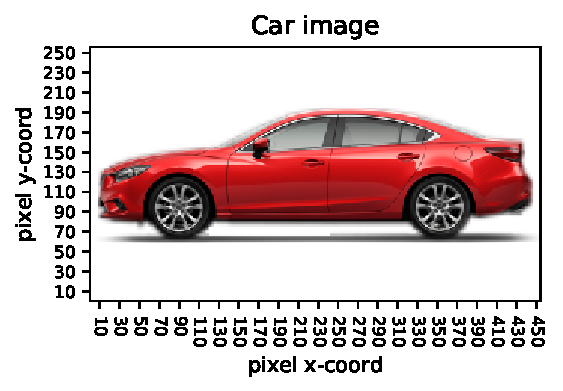
\includegraphics{figs/p2-car.pdf}
\end{figure}

\begin{figure}[!ht]
  \center
  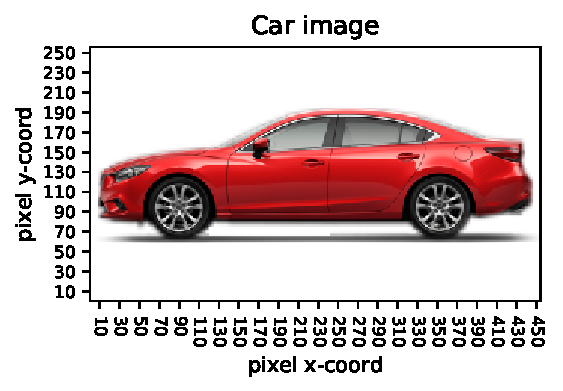
\includegraphics{figs/p2-car-grid.pdf}
\end{figure}

\begin{figure}[!ht]
  \center
  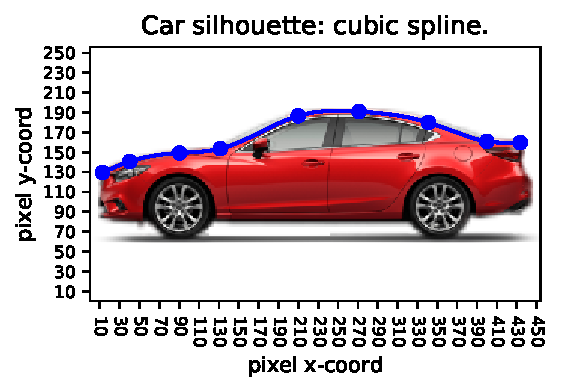
\includegraphics{figs/p2-car-grid-cubic.pdf}
\end{figure}

\verbatiminput{data/points.txt}

\T{2}{Boundary analysis for $\tau$}

  The third property of the tension-spline is defined as:

  \begin{center}
  $
    T''''(x) - \tau^2 \cdot T''(x) = 0 \iff
    T''''(x) = \tau^2 \cdot T''(x)
  $
  \end{center}

  for each $ x \in [x_{i-1},x_i]$. Given $ \tau = 0 $, $T''''(x)$ becomes zero,
  and if $\tau \rightarrow -\infty/\infty$, $T''''(x) \rightarrow \infty$. \\

\T{3}{Construct matrix-vector system and prove solution exists}

  The linear system for variables $z_i$, $i = 0,...,n$ is given by:
  \begin{center}
    $\alpha_{i-1}z_{i-1} + z_i(\beta_{i-1} + \beta_i) + \alpha_i z_{i+1} =
    \gamma_i - \gamma_{i-1}$
  \end{center}

  where;

  \begin{align*}
    h_i &= x_{i+1} - x_i \\
    \alpha_i &= \frac{1}{h_i} - \frac{\tau}{\mathrm{sinh}(\tau h_i)} \\
    \beta_i &= \frac{\tau \mathrm{cosh}(\tau h_i)}{\mathrm{sinh}(\tau h_i)} -
    \frac{1}{h_i} \\
    \gamma_i &= \frac{\tau^2(y_{i+1}-y_i)}{h_i}
  \end{align*}

  Then, iterating over $i$ on the interval $[0,n]$ results in the following set of equations:

  \begin{center}
    $\alpha_{0}z_{0} + z_1(\beta_{0} + \beta_1) + \alpha_1 z_{2} = \gamma_1
    - \gamma_{0}$ \\
    $\vdots$ \\
    $\alpha_{n-2}z_{n-2} + z_{n-1}(\beta_{n-2} + \beta_{n-1}) + \alpha_{n-1}
    z_{n} = \gamma_{n-1} - \gamma_{n-2}$ \\
  \end{center}

  which, written in matrix form become: \\

  $
  \begin{bmatrix}
    \alpha_0 & \beta_0 + \beta_1 & \alpha_1 & 0 & \cdots & 0 \\
    0 & \alpha_1 & \beta_1 + \beta_2 & \alpha_2 & 0 & \\
    \vdots & \ddots & \ddots & \ddots & \ddots &\vdots \\
    0 &  \cdots & 0 & \alpha_{n-2} & \beta_{n-2} + \beta_{n-1} & \alpha_{n-1} & \\
  \end{bmatrix}
  \begin{bmatrix}
    z_0 \\
    \vdots \\
    z_n
  \end{bmatrix}
  =
  \begin{bmatrix}
   \gamma_1 - \gamma_0\\
    \vdots \\
    \gamma_{n-1} - \gamma_{n-2}\\
  \end{bmatrix}
  $ \\

  and with the additional conditions, $z_0 = z_n = 0$: \\ \ \\
  $
  \begin{bmatrix}
  1 & 0 & \cdots & & & 0 \\
  \alpha_0 & \beta_0 + \beta_1 & \alpha_1 & 0 & \cdots & 0 \\
  0 & \alpha_1 & \beta_1 + \beta_2 & \alpha_2 & 0 & \\
  \vdots & \ddots & \ddots & \ddots & \ddots &\vdots \\
  0 &  \cdots & 0 & \alpha_{n-2} & \beta_{n-2} + \beta_{n-1} & \alpha_{n-1} & \\
  0 & \cdots &  & & 0 & 1 \\
  \end{bmatrix}
  \begin{bmatrix}
    z_0 \\
    \vdots \\
    z_n
  \end{bmatrix}
  =
  \begin{bmatrix}
    0\\
   \gamma_1 - \gamma_0\\
    \vdots \\
    \gamma_{n-1} - \gamma_{n-2}\\
    0
  \end{bmatrix}
  $ \\

  In order to prove that this system provides a unique solution to the
  $z$-values, one can show that the coefficient matrix is \textbf{strictly
  diagonally dominant}. A strictly diagonally dominant matrix is defined as a
  matrix where:
  \begin{center}
    $ |a_{ii}| \geq \sum\limits_{j \neq i}{|a_{ij}|}$ for all $i$.
  \end{center}
  Which in this case evaluates to $|\beta_i + \beta_{i+1}| \geq |\alpha_i| +
  |\alpha_{i+1}|$. \\

  Given that $\mathrm{cosh}(x) \geq 1$, the following can be stated regarding
  the magnitudes of $\alpha_i$ and $\beta_i$:
  $
    |\alpha_i| = |-\alpha_i| = |\frac{\tau}{\mathrm{sinh}(\tau h_i)}-
    \frac{1}{h_i} | \leq |\frac{\tau \mathrm{cosh}(\tau h_i)}{\mathrm{sinh}(\tau h_i)} -
    \frac{1}{h_i}| = |\beta_i|
  $.
  Expanding this further gives;
  $
    |\alpha_i| \leq |\beta_i| \Rightarrow |\alpha_i| + |\alpha_{i+1}| \leq
    |\beta_i| + |\beta_{i+1}|
  $
  or
  $
    |\beta_i| + |\beta_{i+1}| \geq |\alpha_i| + |\alpha_{i+1}|
  $. \\

  Since $\tau \geq 0$ (as per definition), $h_i > 0$ (evaluation progresses in positive
  $x$-direction) and $\mathrm{sinh}(x) > 0$ for $x > 0$, it can be assumed that
  $\beta_i > 0$ as long as $\tau > 0$.
  In the specific case, $\tau = 0$, the following relation is true; $|\beta_i| = |-\frac{1}{h_i}| =
  |\frac{1}{h_i}| = |\alpha|$.
  Given $-\frac{1}{h_i} < 0$, it can be assumed that $\beta_i < 0$ for all $i$
  when $\tau = 0$. This means that the sign of $\beta_i$ will always be the
  same for all $i$, which in turn means that $|\beta_i| + |\beta_{i+1}| =
  |\beta_i + \beta_{i+1}|$. \\


  Combining the following results; $ |\beta_i| + |\beta_{i+1}| \geq |\alpha_i|
  + |\alpha_{i+1}| $ and $|\beta_i| + |\beta_{i+1}| =
  |\beta_i + \beta_{i+1}|$ gives the inequality $|\beta_i + \beta_{i+1}| \geq |\alpha_i| +
  |\alpha_{i+1}|$ which proves that the matrix is strictly diagonally dominant
  and that the matrix-vector system will return a unique solution. \\

\T{4}{Additional conditions}


  Update the matrix-vector updated with the additional conditions $T'(x_0) =
  y'_0$ and $T'(x_n) = y'_n$ where $y'_0$ and $y'_1$ are specified through
  input. Taking the derivative of given function $T(x)$ gives:
%  \begin{multline*}
%    T(x) = \frac{
%             z_i\mathrm{sinh}(\tau(x_{i+1}-x)) +
%             z_{i+1}\textrm{sinh}(\tau(x-x_{i}))
%           }
%           {
%             \tau^2\textrm{sinh}(\tau h_i)
%           } +
%           \\
%           +
%           \frac {
%             (y_i-\frac{z_i}{\tau^2})(x_{i+1}-x)+
%             (y_{i+1}-\frac{z_{i+1}}{\tau^2})(x-x_i)
%           }
%           {
%             h_i
%           }
%  \end{multline*}

  \begin{multline*}
    T'(x) =
           \frac{
             -z_i\tau\mathrm{cosh}(\tau(x_{i+1}-x)) +
             z_{i+1}\tau\textrm{cosh}(\tau(x-x_{i}))
           }
           {
             \tau^2\textrm{sinh}(\tau h_i)
           }
           +
           \frac {
             -y_i+\frac{z_i}{\tau^2} +
             y_{i+1}-\frac{z_{i+1}}{\tau^2}
           }
           {
             h_i
           }
           =
           \\
           =
           \frac{
             z_{i+1}\tau\textrm{cosh}(\tau(x-x_{i}))
           }
           {
             \tau^2\textrm{sinh}(\tau h_i)
           }
           -
           \frac{
             z_i\tau\mathrm{cosh}(\tau(x_{i+1}-x))
           }
           {
             \tau^2\textrm{sinh}(\tau h_i)
           }
           +
           \frac {
             -y_i+\frac{z_i}{\tau^2} +
             y_{i+1}-\frac{z_{i+1}}{\tau^2}
           }
           {
             h_i
           }
           \Rightarrow
           \\
           \tau^2T'(x)
           -
           \frac {
             \tau^2(-y_i+\frac{z_i}{\tau^2} +
             y_{i+1}-\frac{z_{i+1}}{\tau^2})
           }
           {
             h_i
           }
           =
           \frac{
             z_{i+1}\tau\textrm{cosh}(\tau(x-x_{i}))
           }
           {
             \textrm{sinh}(\tau h_i)
           }
           -
           \frac{
             z_i\tau\mathrm{cosh}(\tau(x_{i+1}-x))
           }
           {
             \textrm{sinh}(\tau h_i)
           }
           \Rightarrow
           \\
           \tau^2T'(x)
           -
           \frac {
             \tau^2(y_{i+1}-y_i)+z_i-z_{i+1}
           }
           {
             h_i
           }
           =
           \frac{
             z_{i+1}\tau\textrm{cosh}(\tau(x-x_{i}))
           }
           {
             \textrm{sinh}(\tau h_i)
           }
           -
           \frac{
             z_i\tau\mathrm{cosh}(\tau(x_{i+1}-x))
           }
           {
             \textrm{sinh}(\tau h_i)
           }
           \Rightarrow
           \\
           \tau^2T'(x)
           -
           \gamma_i
           =
           \frac{
             z_{i+1}\tau\textrm{cosh}(\tau(x-x_{i}))
           }
           {
             \textrm{sinh}(\tau h_i)
           }
           -
           \frac{
             z_i\tau\mathrm{cosh}(\tau(x_{i+1}-x))
           }
           {
             \textrm{sinh}(\tau h_i)
           }
           \Rightarrow
           \\
           \tau^2T'(x)
           -
           \frac {
             \tau^2(y_{i+1}-y_i)+z_i-z_{i+1}
           }
           {
             h_i
           }
           =
           \frac{
             z_{i+1}\tau\textrm{cosh}(\tau(x-x_{i}))
           }
           {
             \textrm{sinh}(\tau h_i)
           }
           -
           \frac{
             z_i\tau\mathrm{cosh}(\tau(x_{i+1}-x))
           }
           {
             \textrm{sinh}(\tau h_i)
           }
           \Rightarrow
           \\
           \tau^2T'(x)
           -
           \gamma_i
           =
           \frac{
             z_{i+1}\tau\textrm{cosh}(\tau(x-x_{i}))
           }
           {
             \textrm{sinh}(\tau h_i)
           }
           -
           \frac{
             z_i\tau\mathrm{cosh}(\tau(x_{i+1}-x))
           }
           {
             \textrm{sinh}(\tau h_i)
           }
           +
           \frac{z_i}{h_i}
           -
           \frac{z_{i+1}}{h_i}
           \Rightarrow
           \\
           \tau^2T'(x)
           -
           \gamma_i
           =
           z_{i+1}
           (
             \frac{
               \tau\textrm{cosh}(\tau(x-x_{i}))
             }
             {
               \textrm{sinh}(\tau h_i)
             }
             -
             \frac {
               1
             }
             {
               h_i
             }
           )
           +
           z_i
           (
             \frac {
               1
             }
             {
               h_i
             }
             -
             \frac{
               \tau\mathrm{cosh}(\tau(x_{i+1}-x))
             }
             {
               \textrm{sinh}(\tau h_i)
             }
           )
  \end{multline*} \\

  First evaluation is done with $i=0$ and $x=x_0$:

  \begin{align*}
           \tau^2y'_0
           -
           \gamma_0
           &=
           z_{1}
           (
             \frac{
               \tau\textrm{cosh}(\tau(x_0-x_{0}))
             }
             {
               \textrm{sinh}(\tau h_0)
             }
             -
             \frac {
               1
             }
             {
               h_0
             }
           )
           -z_0
           (
             \frac{
               \tau\mathrm{cosh}(\tau(x_{1}-x_0))
             }
             {
               \textrm{sinh}(\tau h_0)
             }
             -
             \frac {
               1
             }
             {
               h_0
             }
           )
           \\
           \tau^2y'_0
           -
           \gamma_0
           &=
           -z_0\beta_0
           +
           z_{1}\alpha_0
  \end{align*}

  Second evaluation with $i=n-1 = \delta$ and $x = x_n$:

  \begin{align*}
           \tau^2y'_n
           -
           \gamma_{\delta}
           &=
           z_{n}
           (
             \frac{
               \tau\textrm{cosh}(\tau(x_n-x_{\delta}))
             }
             {
               \textrm{sinh}(\tau h_{\delta})
             }
             -
             \frac {
               1
             }
             {
               h_{\delta}
             }
           )
           +
           z_{\delta}
           (
             \frac {
               1
             }
             {
               h_{\delta}
             }
             -
             \frac{
               \tau
             }
             {
               \textrm{sinh}(\tau h_{\delta})
             }
           )
           \\
           \tau^2y'_n
           -
           \gamma_{\delta}
           &=
           z_{\delta} \alpha_{\delta}
           +
           z_{n}\beta_{\delta}
           \\
           \tau^2y'_n
           -
           \gamma_{n-1}
           &=
           z_{n-1} \alpha_{n-1}
           +
           z_{n}\beta_{n-1}
  \end{align*}

  Adding new conditions to the matrix-vector system: \\ \ \\
  $
  \begin{bmatrix}
    -\beta_0 & \alpha_0 & 0 & \cdots & & 0 \\
  \alpha_0 & \beta_0 + \beta_1 & \alpha_1 & 0 & \cdots & 0 \\
  0 & \alpha_1 & \beta_1 + \beta_2 & \alpha_2 & 0 & \\
  \vdots & \ddots & \ddots & \ddots & \ddots &\vdots \\
  0 &  \cdots & 0 & \alpha_{n-2} & \beta_{n-2} + \beta_{n-1} & \alpha_{n-1} & \\
  0 & \cdots &  & 0 & \alpha_{n-1} & \beta_{n-1} \\
  \end{bmatrix}
  \begin{bmatrix}
    z_0 \\
    \vdots \\
    z_n
  \end{bmatrix}
  =
  \begin{bmatrix}
    \tau^2y'_0-\gamma_0 \\
   \gamma_1 - \gamma_0\\
    \vdots \\
    \gamma_{n-1} - \gamma_{n-2}\\
    \tau^2y'_n-\gamma_{n-1}\\
  \end{bmatrix}
  $ \\ \ \\

\T{5}{Fit 10 values derived from cos($x$)}

  \begin{figure}[!ht]
    \center
    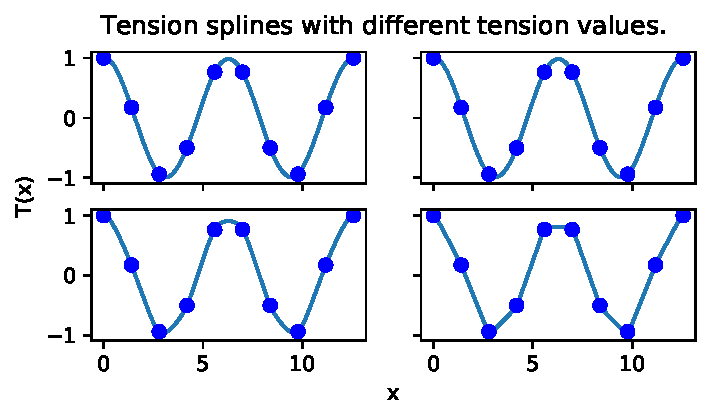
\includegraphics{figs/p2-fit-10-points.pdf}
  \end{figure}

\T{6}{Plot top of car}

  \begin{figure}[!ht]
    \center
    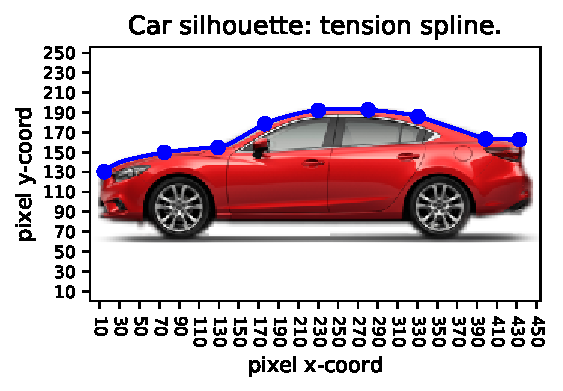
\includegraphics{figs/p2-car-tension-splines.pdf}
  \end{figure}


\end{document}
